\documentclass[conference]{IEEEtran}
\IEEEoverridecommandlockouts
% The preceding line is only needed to identify funding in the first footnote. If that is unneeded, please comment it out.
\usepackage{cite}
\usepackage{amsmath,amssymb,amsfonts}
\usepackage{algorithmic}
\usepackage{graphicx}
\usepackage{textcomp}
\usepackage{xcolor}
\usepackage{tabularray}
\def\BibTeX{{\rm B\kern-.05em{\sc i\kern-.025em b}\kern-.08em
    T\kern-.1667em\lower.7ex\hbox{E}\kern-.125emX}}
\begin{document}

\title{Conference Paper Title*\\
{\footnotesize \textsuperscript{*}Note: Sub-titles are not captured in Xplore and
should not be used}
\thanks{Identify applicable funding agency here. If none, delete this.}
}

% \author{\IEEEauthorblockN{1\textsuperscript{st} Given Name Surname}
% \IEEEauthorblockA{\textit{dept. name of organization (of Aff.)} \\
% \textit{name of organization (of Aff.)}\\
% City, Country \\
% email address or ORCID}
% \and
% \IEEEauthorblockN{2\textsuperscript{nd} Given Name Surname}
% \IEEEauthorblockA{\textit{dept. name of organization (of Aff.)} \\
% \textit{name of organization (of Aff.)}\\
% City, Country \\
% email address or ORCID}
% \and
% \IEEEauthorblockN{3\textsuperscript{rd} Given Name Surname}
% \IEEEauthorblockA{\textit{dept. name of organization (of Aff.)} \\
% \textit{name of organization (of Aff.)}\\
% City, Country \\
% email address or ORCID}
% \and
% \IEEEauthorblockN{4\textsuperscript{th} Given Name Surname}
% \IEEEauthorblockA{\textit{dept. name of organization (of Aff.)} \\
% \textit{name of organization (of Aff.)}\\
% City, Country \\
% email address or ORCID}
% \and
% \IEEEauthorblockN{5\textsuperscript{th} Given Name Surname}
% \IEEEauthorblockA{\textit{dept. name of organization (of Aff.)} \\
% \textit{name of organization (of Aff.)}\\
% City, Country \\
% email address or ORCID}
% \and
% \IEEEauthorblockN{6\textsuperscript{th} Given Name Surname}
% \IEEEauthorblockA{\textit{dept. name of organization (of Aff.)} \\
% \textit{name of organization (of Aff.)}\\
% City, Country \\
% email address or ORCID}
% }
\title{Wireless Capsule Endoscopy Image Super Resolution using Deep Learning}
\maketitle

\section{Experimental Results}
\subsection{Comparision with state-of-the-art models.}

For visualization of statistical analysis we have used boxplots which demonstrates a box between 25\% and 75\% values and other values are known as outliers which are defined by circles below the higher quartile of the boxplot. So for a model to be statistically stable and consistent, the box's size should be as small as possible and also number of outliers should be low as well while the median should be high. We have conducted statistical analysis on PSNR and SSIM values for RGB and Y channel both as shown in Fig. [\ref{PSNR:RGB}-\ref{SSIM:Y}]. It can be observed from boxplot images that DCAN has the smallest size of the quartile box and lowest number of outliers with having high median among all the models. 
\begin{figure*}[h!]
  \centering
  \begin{minipage}{0.3\textwidth}
    \centering
    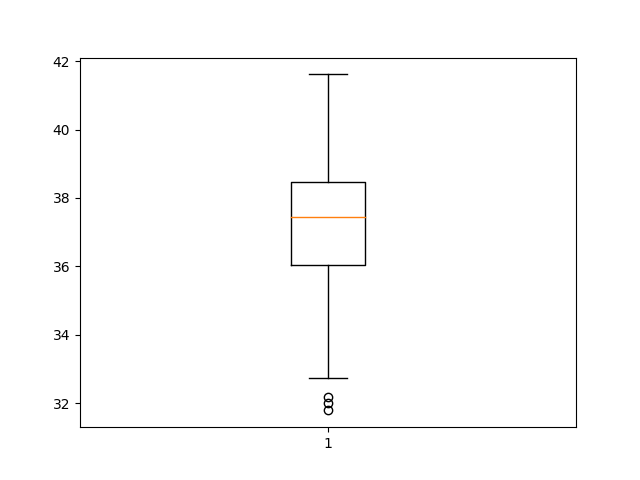
\includegraphics[width=\textwidth,height=0.2\textheight]{bicubic_rgb.png}
    (a) Bicubic
    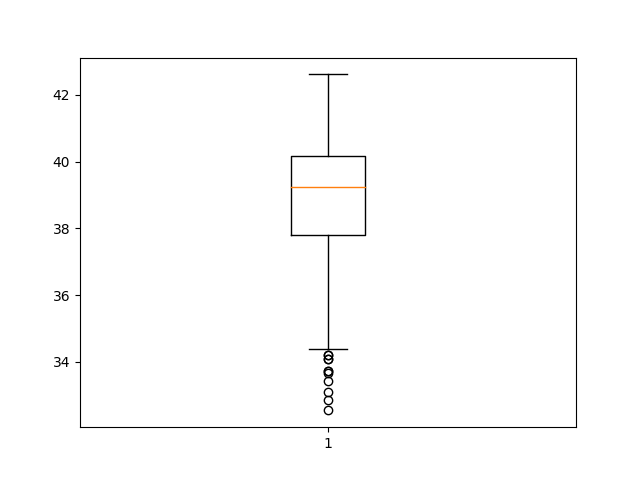
\includegraphics[width=\textwidth,height=0.2\textheight]{dense_rgb (1).png}
    (d) DenseNet
  \end{minipage}%
  \begin{minipage}{0.3\textwidth}
  \centering
  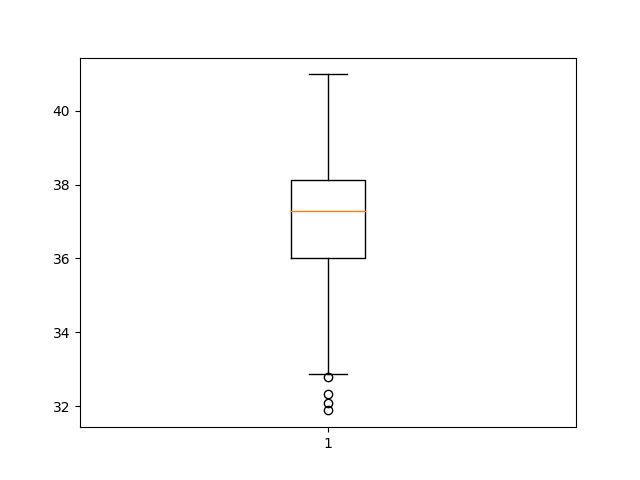
\includegraphics[width=\textwidth,height=0.2\textheight]{srgan_rgb.png}
   (b) SRGAN
  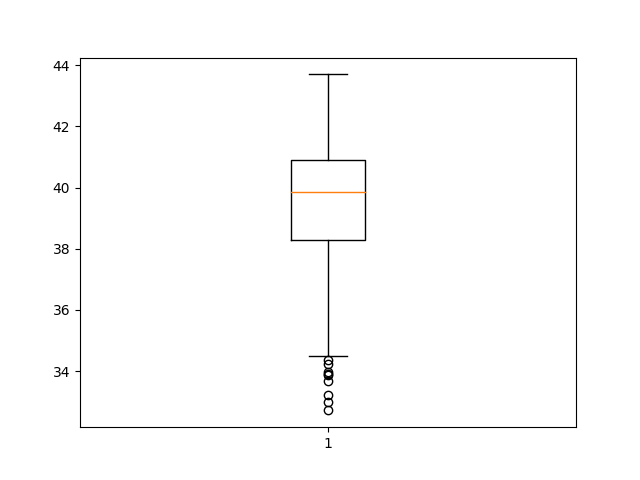
\includegraphics[width=\textwidth,height=0.2\textheight]{rcan_rgb.png}
   (e) RCAN 
  \end{minipage}%
  \begin{minipage}{0.3\textwidth}
  \centering
  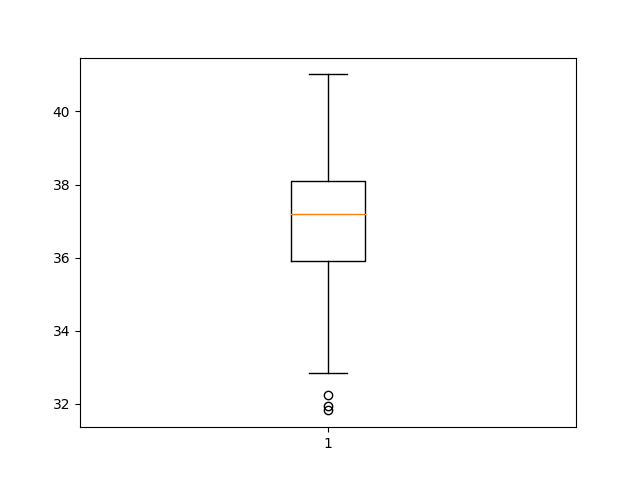
\includegraphics[width=\textwidth,height=0.2\textheight]{Figures/cyclegan_rgb.png}
  (c) CycleGAN 
  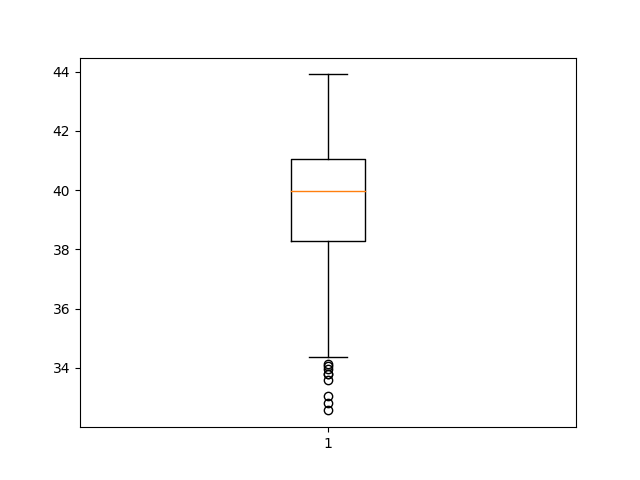
\includegraphics[width=\textwidth,height=0.2\textheight]{proposed_rgb.png}
  (f) DCAN(ours)
  \end{minipage}%
  \caption{PSNR comparision of all models using box plots in RGB channel}
  \label{PSNR:RGB}
  \end{figure*}


\begin{figure*}[h!]
  \centering
  \begin{minipage}{0.3\textwidth}
    \centering
    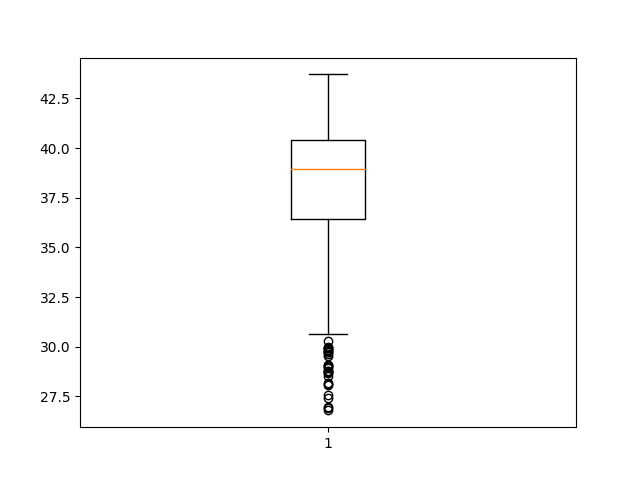
\includegraphics[width=\textwidth,height=0.2\textheight]{bicubic_y.png}
    (a) Bicubic
    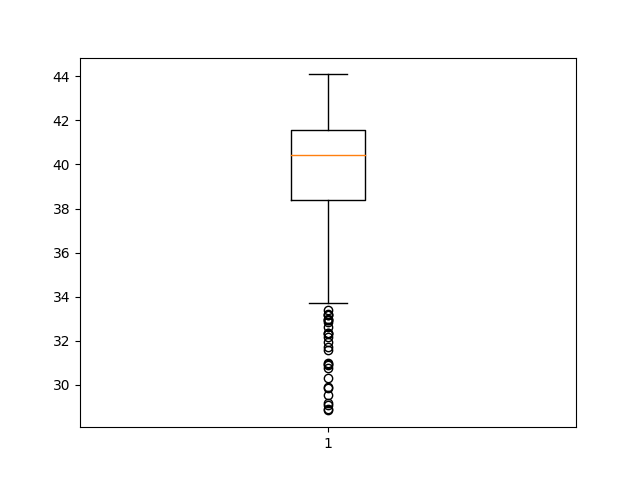
\includegraphics[width=\textwidth,height=0.2\textheight]{dense_y (1).png}
    (d) SR DenseNet 
  \end{minipage}%
  \begin{minipage}{0.3\textwidth}
  \centering
  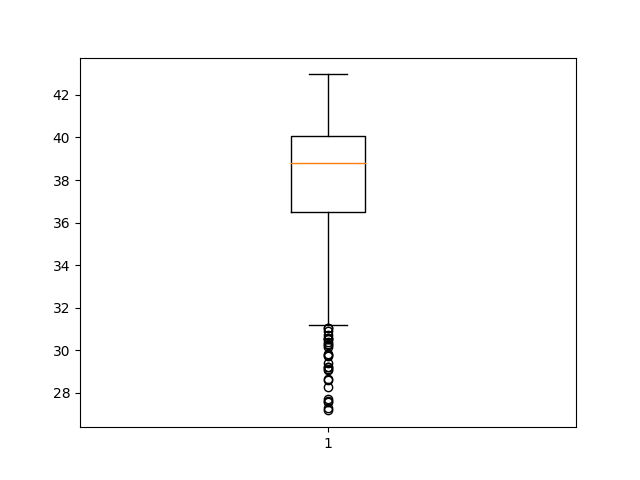
\includegraphics[width=\textwidth,height=0.2\textheight]{srgan_y (1).png}
  (b) SRGAN 
  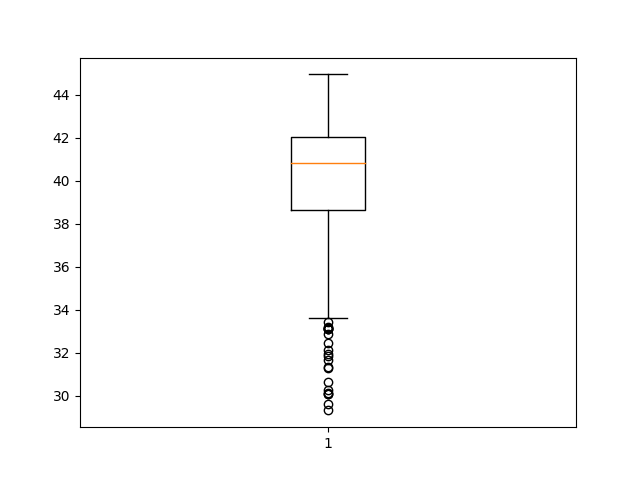
\includegraphics[width=\textwidth,height=0.2\textheight]{rcan_y (2).png}
  (e) RCAN
  \end{minipage}%
  \begin{minipage}{0.3\textwidth}
  \centering
  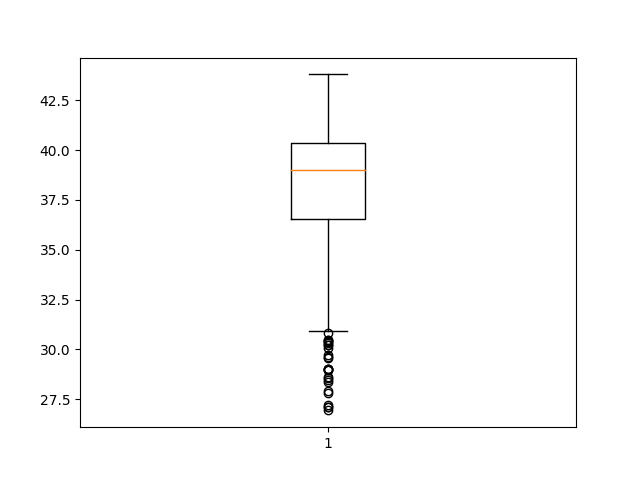
\includegraphics[width=\textwidth,height=0.2\textheight]{Figures/cyclegan_y.png}
  (c) CycleGan 
  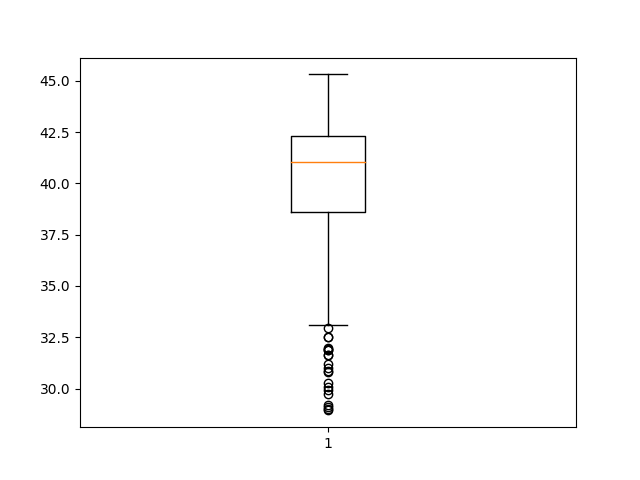
\includegraphics[width=\textwidth,height=0.2\textheight]{proposed_y (2).png}
  (f) DCAN(ours)
  \end{minipage}%
  \caption{PSNR comparision of all models using box plots in Y channel}
  \label{PSNR:Y}
  \end{figure*}

\begin{figure*}[h!]
  \centering
  \begin{minipage}{0.3\textwidth}
    \centering
    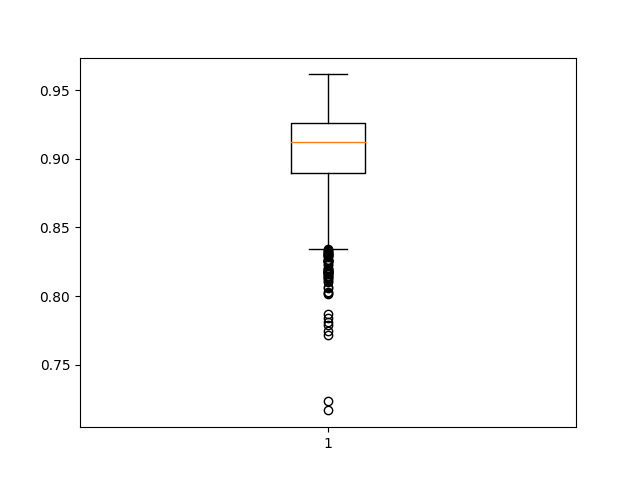
\includegraphics[width=\textwidth,height=0.2\textheight]{Figures/bicubic_ssim_rgb.png}
    (a) Bicubic
    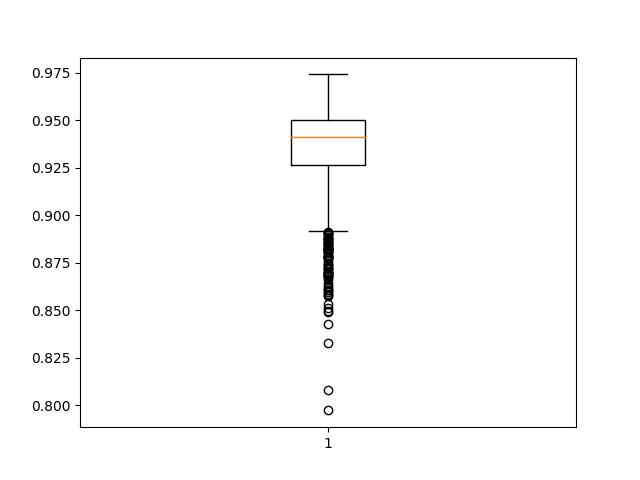
\includegraphics[width=\textwidth,height=0.2\textheight]{Figures/dense_ssim_rgb.png}
    (d) SR DenseNet
  \end{minipage}%
  \begin{minipage}{0.3\textwidth}
  \centering
  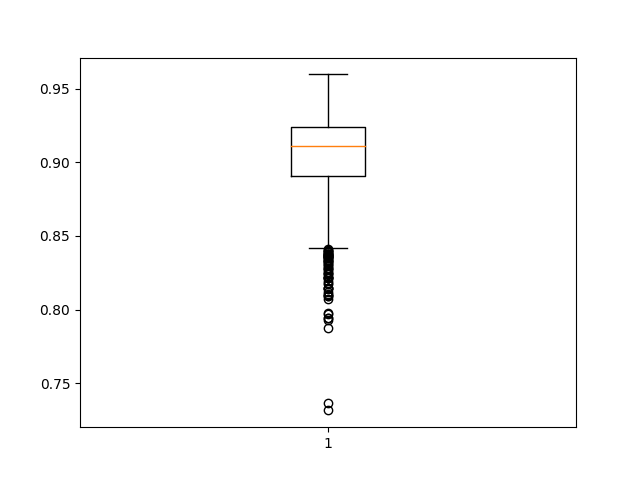
\includegraphics[width=\textwidth,height=0.2\textheight]{Figures/srgan_ssim_rgb.png}
  (b) SRGAN 
  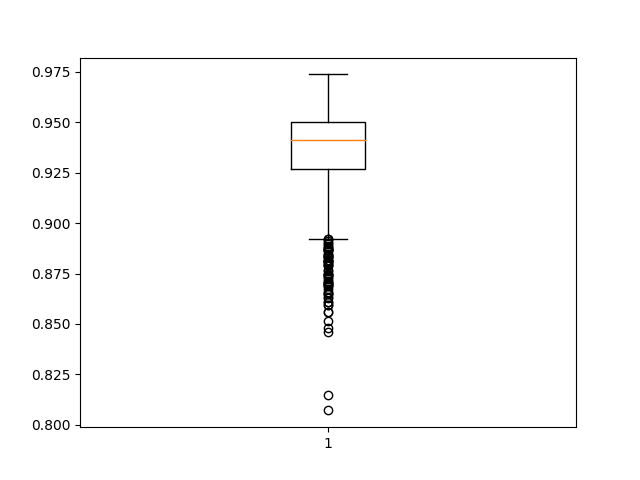
\includegraphics[width=\textwidth,height=0.2\textheight]{Figures/rcan_ssim_rgb.png}
  (e) RCAN 
  \end{minipage}%
  \begin{minipage}{0.3\textwidth}
  \centering
  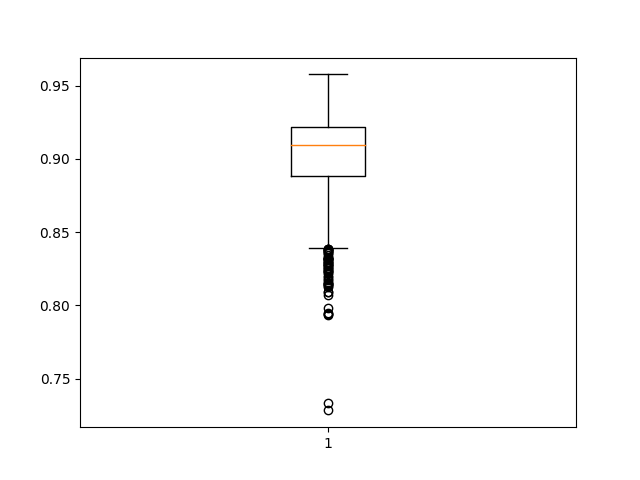
\includegraphics[width=\textwidth,height=0.2\textheight]{Figures/cyclegan_ssim_rgb.png}
  (c) CycleGAN 
  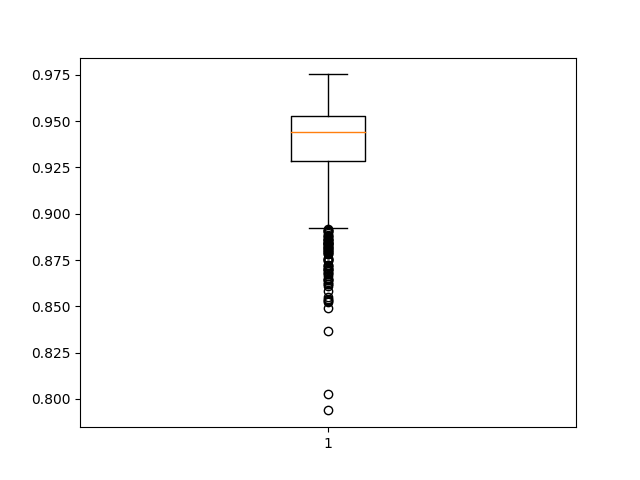
\includegraphics[width=\textwidth,height=0.2\textheight]{Figures/proposed_ssim_rgb.png}
  (f) DCAN(ours)
  \end{minipage}%
  \caption{SSIM comparision of all models using box plots in RGB channel}
  \label{SSIM:RGB}
  \end{figure*}
  
\begin{figure*}[h!]
  \centering
  \begin{minipage}{0.3\textwidth}
    \centering
    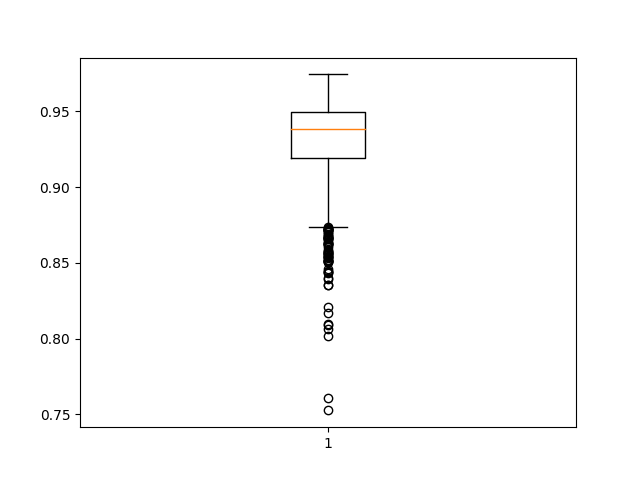
\includegraphics[width=\textwidth,height=0.2\textheight]{Figures/bicubic_ssim_Y.png}
    (a) Bicubic
    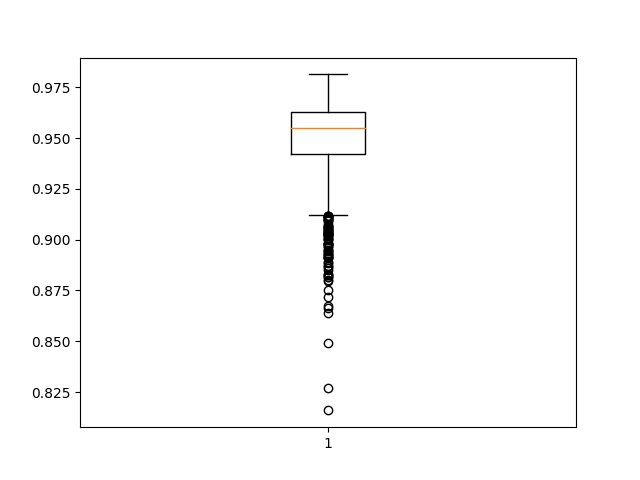
\includegraphics[width=\textwidth,height=0.2\textheight]{Figures/dense_ssim_Y.png}
    (d) SR DenseNet 
  \end{minipage}%
  \begin{minipage}{0.3\textwidth}
  \centering
  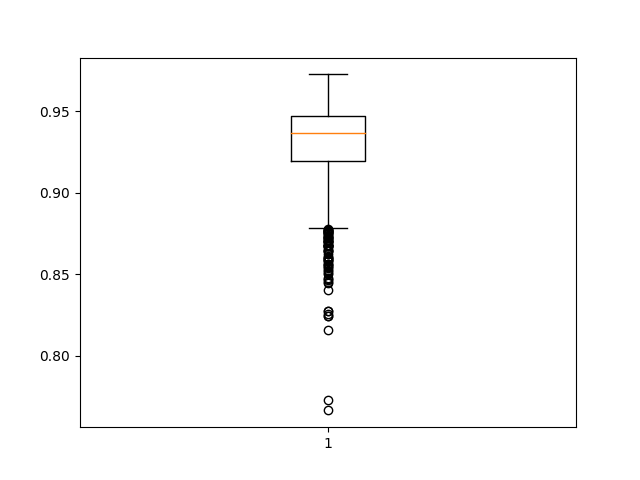
\includegraphics[width=\textwidth,height=0.2\textheight]{Figures/srgan_ssim_Y.png}
  (b) SRGAN 
  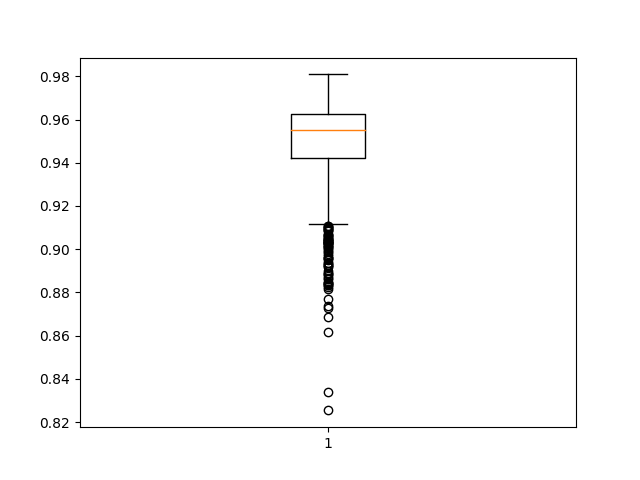
\includegraphics[width=\textwidth,height=0.2\textheight]{Figures/rcan_ssim_Y.png}
  (e) RCAN 
  \end{minipage}%
  \begin{minipage}{0.3\textwidth}
  \centering
  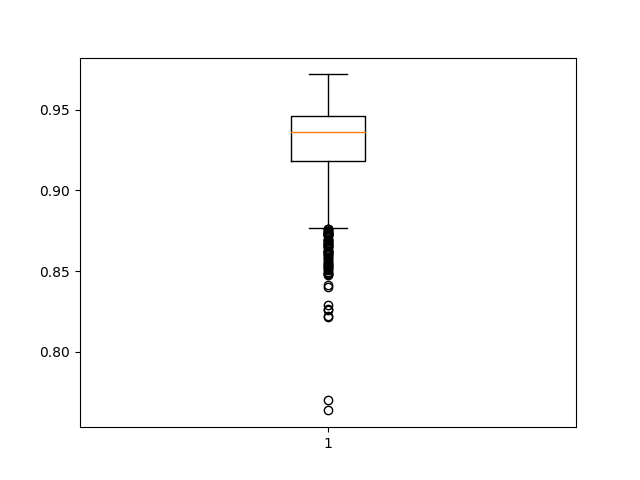
\includegraphics[width=\textwidth,height=0.2\textheight]{Figures/cyclegan_ssim_Y.png}
  (c) CycleGAN
  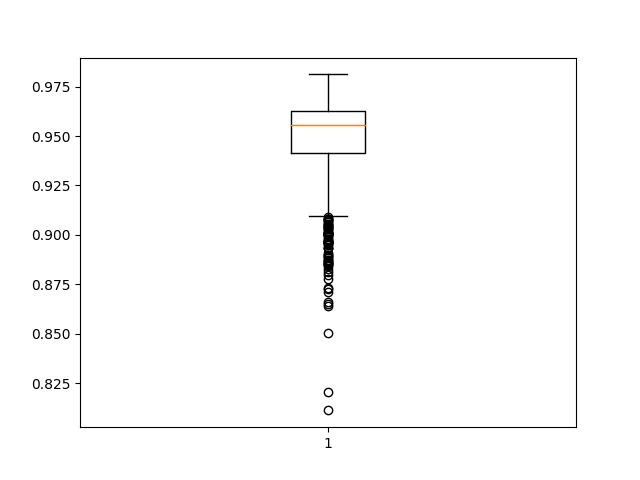
\includegraphics[width=\textwidth,height=0.2\textheight]{Figures/proposed_ssim_Y.png}
  (f) DCAN(ours)
  \end{minipage}%
  \caption{SSIM comparision of all models using box plots in Y channel}
  \label{SSIM:Y}
  \end{figure*}

  \end{document}
